In this chapter we will discuss the implementation on various modules of the \sys\ architecture. We start off by describing all the components we worked on and then explain in detail the parts which are relevant to this thesis.

\section{Parts of the \sys\ Architecture}

We have created multiple modules, each with a different functionality and objective. We list the major modules in the \sys\ architecture below:

\begin{enumerate}
	\item \textbf{Main Controller} - T
	\item \textbf{Data Loader} - 
	\item \textbf{Data Batcher}
	\item \textbf{Memory Network}
	\item \textbf{Dynamic Decoder}
	\item \textbf{Attention Mechanism}
	\item \textbf{Beam Search}
	\item \textbf{Evaluator}
	\item \textbf{Logging}
\end{enumerate}

We depict the interaction between the multiple components in Figure \ref{fig:sys_comp}. The components with a blue shade will be covered in the scope of this thesis.

\begin{figure}[!ht]
\centering
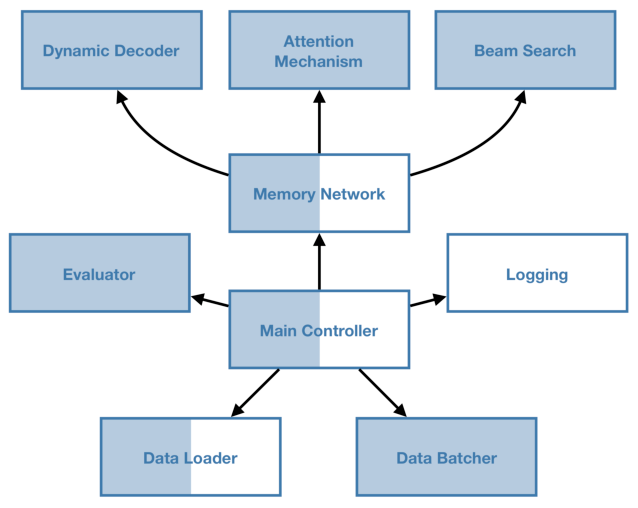
\includegraphics[scale=1.0]{assets/figures/components_orig.pdf}
\caption{(a) an example dialog with history and KB tuples. (b) an illustration of Mem2Seq memory. (c) an illustration of \sys\ memory}
\label{fig:sys_comp}
\end{figure}

\noindent\textbf{Main Controller}

\noindent\textbf{Data Loader}

\noindent\textbf{Data Batcher}

\noindent\textbf{Memory Network}

\noindent\textbf{Dynamic Decoder}

\noindent\textbf{Attention Mechanism}

\noindent\textbf{Beam Search}

\noindent\textbf{Evaluator}

\section{Parts of the \sys\-RL Architecture}

There are mainly three main components that have been added to the \sys\ architecture to make \sys -RL. These are listed below.

\begin{enumerate}
	\item \textbf{API Explorer} - This systematically searches the space of APIs and populates the buffer to be used by MAPO.
	\item \textbf{Rewards} - This takes in a particular API as input along with the expected future responses and returns the reward/pseudo-reward.
	\item \textbf{RL-Decoder} - This is the main API generator which we train to learn the ideal policy.
	\item \textbf{Augmented REINFORCE} - This takes in results from both the API explorer populated buffer and the RL-decoder outputs and runs Augmented REINFORCE (MAPO) on top of them.
\end{enumerate}

We observe the interaction between these added components and the previous architecture in Figure \ref{fig:sys_comp_rl}.

\begin{figure}[t]
\centering
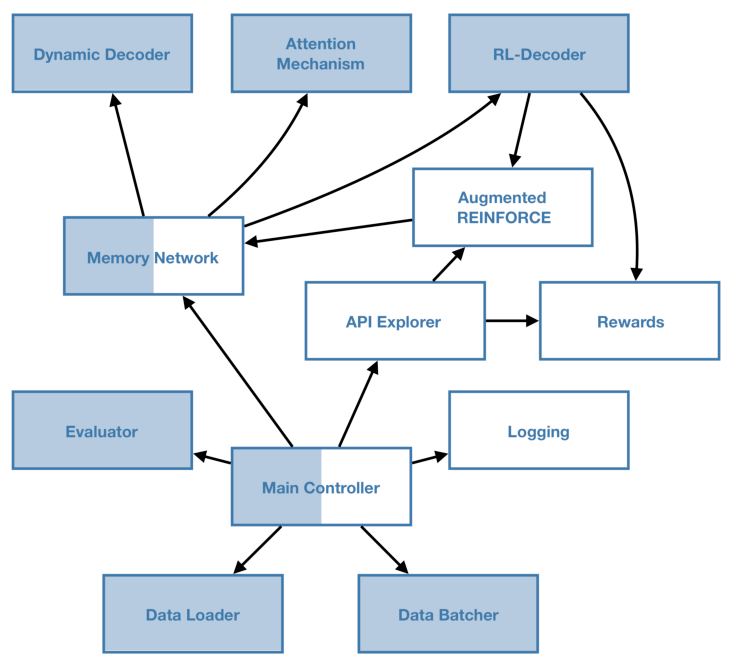
\includegraphics[scale=1.2]{assets/figures/rl_components.pdf}
\caption{(a) an example dialog with history and KB tuples. (b) an illustration of Mem2Seq memory. (c) an illustration of \sys\ memory}
\label{fig:sys_comp_rl}
\end{figure}

\noindent\textbf{Main Controller}

There are several changes that had to be made to the main controller to handle the RL-decoding policy. First, we implemented a phase-wise training to help enable the RL-decoder and the response model to train independently. In this phase we have 4 phases:
\begin{enumerate}
	\item \textbf{Phase 1} : This trains the response deocder only for dialogs that occur before any API is made.
	\item \textbf{Phase 2} : This phase adds in the training for the RL-decoder. This is only used in case we use a shared embedding space for encoding the context for the response deocder and RL-decoder. If they use different embeddings, then Phase 2 can be directly merged with Phase 1.
	\item \textbf{Phase 3} : In this phase we can now start training the system on responses after the API call has been made. We include the results retrieved by the RL-decoder in Phase 2.
	\item \textbf{Phase 4} : This phase calculates the actual reward based on the responses innn Phase 3 and retrains the RL-decoder accordinly. This reward actually measures how well the system was able to train on the retrieved results and will be able to capture the effects of how the results are stored in memory, like sorting based on a field.
\end{enumerate}

These phases are run one after the other and more phases are activated after the previous phases near convergence. For example we start off with just Phase 1 and after it converges we now run Phase 1 and 2 together.

\noindent\textbf{Memory Network}

We added three main APIs in the memory network to enable the RL-decoder. 

\begin{itemize}
	\item \emph{api\_predict} will attempt to predict good API responses via the RL-decoder policy and utilises beam search to get a large set predictions.
	\item \emph{api\_train} takes in APIs and their rewards and then implements the augmented REINFORCE algorithm
	\item \emph{api\_prob} takes in an API and returns the probability of generating that API with the current policy.
\end{itemize}

\noindent\textbf{RL-Decoder}

The RL-decoder takes in the encoded state as the inital state. It maintains a time variable which corresponds to the current time step of the decoder. This time variable is sent through a position embedding and is then sent as input to the decoder. We set the next state of the decoder as the inital state so that we break the sequential behavior as required. This decoder uses the dynamic decoder with beam search to decode and attends over the input context via the attention wrapper.
